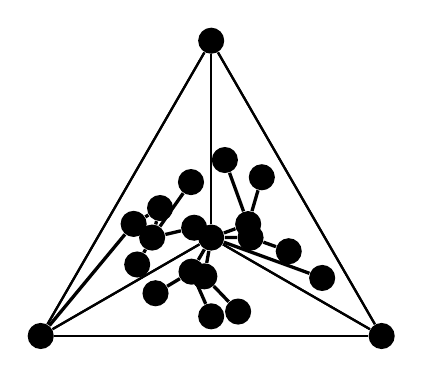
\begin{tikzpicture}[scale = 0.5]
    \foreach \angle in {0,...,2} {
        \node[fill, circle] (shell\angle) at (90+\angle*120:5) {};
    }
    \node[fill,circle] (shell3) at (0,0) {};
    \foreach \i in {0,...,3} {
        \foreach \j in {0,...,3} {
            \draw[thick] (shell\i) -- (shell\j);
        }
    }

    \node[fill, circle, \clrone] (1) at (90+60:.5) {};
    \node[fill, circle, \clrone] (2) at (90+90:1.5) {};
    \node[fill, circle, \clrone] (3) at (90+20:1.5) {};
    \node[fill, circle, \clrone] (4) at (90+60:1.5) {};
    \node[fill, circle, \clrone] (5) at (90+80:2) {};
    \node[fill, circle, \clrone] (6) at (90+110:2) {};
    
    \node[fill, circle, \clrone] (7) at (210+30:1) {};
    \node[fill, circle, \clrone] (8) at (210+50:1) {};
    \node[fill, circle, \clrone] (9) at (210+15:2) {};
    \node[fill, circle, \clrone] (10) at (210+60:2) {};
    \node[fill, circle, \clrone] (11) at (210+80:2) {};
    
    \node[fill, circle, \clrone] (12) at (330+30:1) {};
    \node[fill, circle, \clrone] (13) at (330+50:1) {};
    \node[fill, circle, \clrone] (14) at (330+20:2) {};
    \node[fill, circle, \clrone] (15) at (330+10:3) {};
    \node[fill, circle, \clrone] (16) at (330+80:2) {};
    \node[fill, circle, \clrone] (17) at (330+110:2) {};

    \draw[very thick, \clrtwo] (shell3) -- (1) -- (2) -- (3) (2) -- (4) -- (5) (2) -- (6) (shell3) -- (7) -- (9) (7) -- (10) (shell3) -- (8) -- (11) (shell3) -- (12) -- (14) (shell3) -- (15) (shell3) -- (13) -- (16) (13) -- (17);

    \draw[very thick, \clrtwo] (5) -- (shell1);


\end{tikzpicture}